\chapter{How to Begin}
This part might go in Chapter 1???

\section{Design Progression}
While it may be tempting to attack a design problem with all of the computational tools at your disposal, that may not be the best approach. Informed decisions at the beginning of the project reduce the amount of work that you and your computer will have to do. 
In general, low-fidelity methods or formulations are entirely satisfactory at the start. Simple calculations also tend to provide understanding and intuition that will be useful as the design process continues.

\begin{figure}[!hb]
  \label{fig:linear_design}
  \centering
  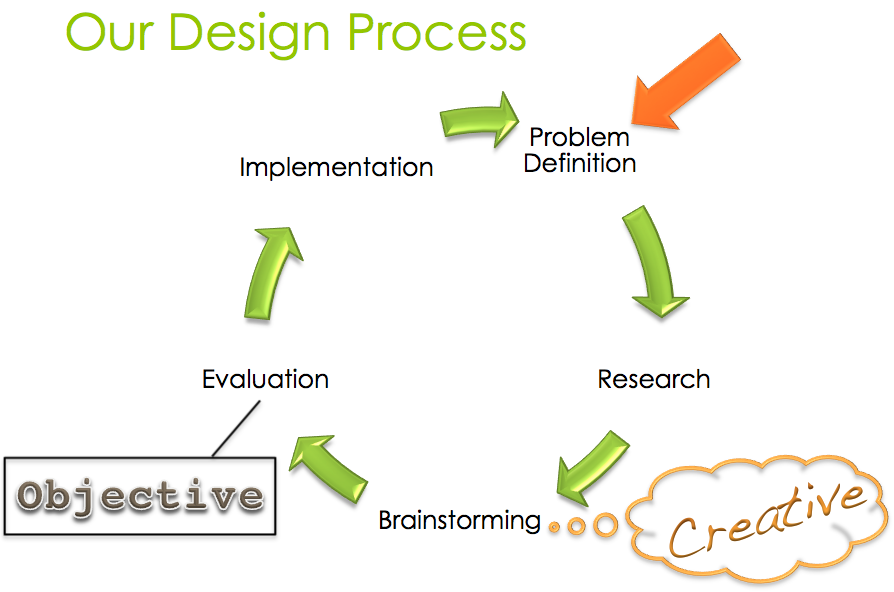
\includegraphics[width=0.75\textwidth]{graphics/design_process_big.png}
  \caption{Simplified design process. (Graphic from http://ahmackenziedesign.com/faq/ )}
\end{figure}

As the design matures, so should the tools being used. Think of computer codes as sieves. Low-fidelity codes will filter out designs that obviously won't work and more sophisticated tools may be needed to decide between closely competing design alternatives.

\begin{wrapfigure}{R}{0.375\textwidth}
  \label{fig:cluttered_design}
  \centering
  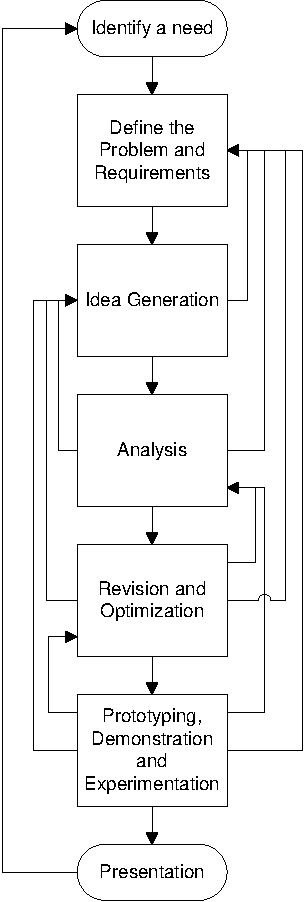
\includegraphics[width=0.35\textwidth]{graphics/GeneralDesignProcess_cluttered.pdf}
  \caption{Realistic design process.}
\end{wrapfigure}

That being said, the ultimate goal is to reduce the time needed to generate a satisfactory design. There is no reason to spend more time on a less accurate method. For example, spending an hour to calculate the four-factor formula by hand with analytical methods is not as wise as waiting 15 minutes for the results from a Monte Carlo simulation. So the rough-cut tools you use should also be fast and easy to use.

While it is easier to describe a linear design process, that is usually not how it works in practice. Initially there will likely be several candidate designs which should be investigated in parallel. The number of competing designs will decrease as time goes on. 
Furthermore, design textbooks generally present the design process as a chronological journey through a serious of tasks (Figure~\ref{fig:linear_design}). But this is not accurate, because design is an iterative process. So then the flow charts are given arrows for every point to every preceding point, as in Figure~\ref{fig:cluttered_design}. 
With such a tangled picture in mind, we wish to emphasize from the outset that the design process will involve regular backtracking, especially since ideas are not generated only during brainstorming sessions.
The important thing is keep moving and maintain a willingness to backtrack, modify, and change your design. Trying to design an optimal reactor from the outset will certainly lead to slow going. So do your best to stay out of rabbit holes at the beginning and leave the details for later.


\section{Initial Decisions}
Decisions made at the beginning of the design process have a bigger effect on life cycle costs than decisions made toward the end as shown in Figure~\ref{fig:life_cycle_cost}. 
As time goes on, certain design commitments have been made and retroactive actions are more costly than designing it right the first time.
Clearly, proper engineering design which takes full account of all foreseeable problems will greatly reduce the cost of the project.
Furthermore, the front end of the design phase is also important. So it is worthwhile to carefully examine all of the options available at the beginning of the project. 

Some decisions can be made immediately based on engineering knowledge and an understanding of the design goals. Two of the most generic questions are What enrichment is acceptable? and What energy spectrum should the reactor have? The constraint of using natural uranium will quickly suggest a thermal reactor with only a few options for moderators. The desire to breed plutonium will dictate a high-neutron energy spectrum. 

\begin{figure}[!hbp]
  \label{fig:life_cycle_cost}
  \centering
  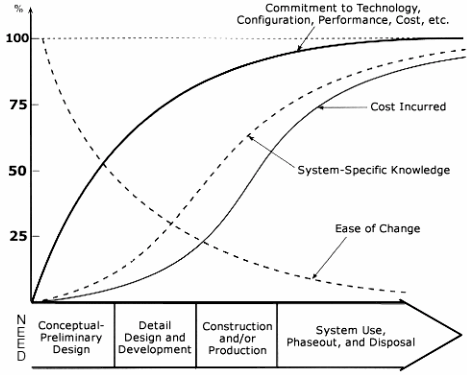
\includegraphics[width=0.70\textwidth]{graphics/life_cycle_cost_chart.png}
  \caption{Commitment, system-specific knowledge, and cost (source: B.S. Blanchard \& W.J. Fabrycky, Systems Engineering and Analysis, 3rd Ed., Prentice Hall, 1998, Figure 2.11).}
  %http://www.sole.or.kr/Download/SOLEtech/SOLEtech(Volume%204.12).htm
\end{figure}

After the obvious choices have been made, but without accidentally eliminating any viable choices, there are a few fundamental decisions to make. The choice of moderator (if needed), coolant, fuel isotope, and chemical fuel form are the fundamental features around which the reactor will be designed. These decisions do not require any computer simulations if the correct figures of merit are identified and used. 

Often selection is not straightforward because the materials are better at some things and worse in other respects. In cases like these, the decision is which set of issues you want to deal with.
The way each issue is weighted will influence the decision. For example, if low R\&D requirements is a priority, UO$_2$ will be selected and the poor thermal conductivity will have to be dealt with. 
Dichotomies like this help explain why there remains such a diversity of opinions and research efforts.
In other words, there may be more than one acceptable answer, but it is important to explain why the selection was made.

% Chris will probably want to expand this part quite a bit

\subsection{Coolant Selection}
Nuclear engineers often think of neutronic design as the critical (pun intended) part of the reactor system. However, neutron transport is actually a smaller part of the design than one would think.
In any reactor that produces power, cooling is essential. When the goal is producing electricity, managing the working fluid is the key to reliability and efficiency. Thus we begin with a discussion of coolants.

The first question is, Is this a thermal spectrum reactor? If the answer is no, many low-Z coolants are automatically eliminated from consideration.
Next, the desired operating temperatures need to be assigned ballpark numbers. This is determined by estimating the capabilities of heat exchangers, turbo-machinery, and structural and piping materials. You can prescribe these limits later if necessary, remember design is an iterative process. 

The following coolant properties are desirable for any reactor. \emph{High heat capacity}. This allows the coolant to absorb more energy per change in temperature. \emph{Non-corrosive}. Whatever the coolant contacts, or has the potential to contact, it should be compatible with. If the coolant corrodes the cladding, it will limit the fuel cycle length and sabotage the fuel utilization. \emph{Radiation stability} The coolant in the core will experience high radiation fields and radiolysis and neutron activation will occur. The coolant should be selected so that these phenomena are minimized. \emph{Low cross section} Neutrons absorbed in the coolant or coolant impurities will diminish the performance of the reactor \cite{Hausner}.

%water
% liquid metal
% gas
% salts
% other

\subsubsection{Comparison of Liquid and Gaseous Coolants}
The phase of the coolant is an important consideration. Both liquid and gaseous coolants have their advantages and disadvantages.
If gaseous coolant is chosen, the chemically inert noble gases become attractive options.

\begin{table}[!ht]
\begin{tabular}{c|c|c|c}
  Qualtiy & Liquid & Two-Phase & Gaseous \\
  \hline
  Heat Capacity & High & High & Low \\
  Phase Change & Limiting condition & Desirable & Not an issue \\
  Heat Transfer Coefficient & High & Very high & Low \\
  Natural Circulation & Good & Very good & Poor \\
  Pumping Power & Low/good & Low/good & High/bad\\
  Neutron Absorption & High & Less & Low\\
  Direct Cycle & No & Yes, Rankine & Yes, Brayton\\
  Low Pressure & Maybe & No & No\\
  %
  \hline
\end{tabular}
\caption{Phase of coolant}
\end{table}

%\subsubsection{Comparison of Molten Salts and Liquid Metals}
%\subsubsection{Comparison of Moderating Coolants}
% or:
%\subsubsection{Comparison of Liquid Coolants}


\subsection{Moderator Selection}
For thermal reactors, a low-Z element is needed to slow down the fission neutrons to low energy levels where fission is more likely to occur. It must also do this without absorbing too many neutrons. Hydrogen is an obvious choice because of its ability to stop a neutron completely with only one scattering interaction and its low mean free path. Deuterium comes to mind next because it absorbs neutrons 1000 times less. Graphite is a desirable moderator because it can withstand extremely high temperatures.
%reproduce Duderstadt discussion and table

% \subsection{Figures of Merit}

\subsection{Fuel Selection}
The requirements of nuclear fuel are very demanding due to the environment it must withstand. Hausner \cite{Hausner}
lists the following requirements for nuclear fuel
\begin{itemize}
\item[1.] It must be able to tolerant radiation damage
\item[2.] It must not corrode upon contact with the cladding or coolant.
\item[3.] It or its impurities must not absorb too many neutrons
\item[4a.] It must be able to withstand the temperature gradient caused by the heat it generates
\item[4b.] It should have high thermal conductivity (or appropriate dimensions) in order to transmit its heat to the coolant
\item[5.] It must be able to withstand the thermal cycles that it will experience during operation
\item[6.] It must be able to withstand the mechanical loads placed upon it
\item[7.] It must be inexpensive
\item[8.] It should lend itself to the fuel cycle in which it will be used, e.g. easy to reprocess
\end{itemize} 

Also it is generally preferable to have a high density in order to ease requirements for enrichment.

\subsection{Cladding Selection}
Material selection for cladding is important because it is the first line of defense for retaining radioactive material.
Even for reactor designs with no cladding, e.g. a molten salt-fueled reactor, it is necessary to select compatible and durable materials to contain the nuclear material and working fluid.
Selecting reliable cladding and piping materials allows the reactor to run smoothly with fewer interruptions. The primary requirement is for the cladding to be chemically compatible with both the fuel and the coolant. Superior corrosion performance is the foremost concern.

The cladding material must also be capable of enduring an extreme environment of neutron, gamma, and fission product irradiation and high temperatures. It must also maintain its strength and ductility while absorbing as few as possible neutrons. 
After all this, it would be preferable if the material was cheap and easy to manufacture.

\subsection{Secondary Circuit Working Fluid Selection}
For power reactors that do not use a direct cycle, a working fluid in the secondary system must be selected. Generally the working fluid for energy conversion can be selected after the primary coolant has been determined. 
However, the potential secondary fluids may weigh on the decision of the primary fluid.
For example, sodium coolant may be disfavored because of its incompatibility with water. 
But for most other coolants the choice is not as important. 

Water is by far the most used working fluid for nuclear reactors. Even sodium-cooled reactors have converted energy with a steam system (making the complexity of intermediate loops and pipe-in-pipe heat exchangers necessary). 
The widespread use of steam turbines has made that power conversion system quite familiar.

Several advanced reactor concepts call for the use of the Brayton cycle with Helium or super-critical CO$_2$ as the working fluid. These systems can (must) work at higher temperatures and they achieve higher efficiency.

% talk about why a Mercury Rankine cycle is not very good.

\section{Geometric Specification}
After these have been determined, the basic core geometry comes next. 
At this point an optimized design is unlikely and even unneeded. More likely each analysis will provide the limits of a feasible design space. 

There are several options for fuel layout: pins, plates, fluid, and dispersion.
For optimal neutronics performance, the percentage of cladding material must be reduced. Thus large fuel pins are favored.
From the heat transfer perspective the surface area of the fuel per volume should be maximized. This pushes the design towards plate fuel.
These competing requirements will lead to trade-offs and constraints.

Dispersion fuels such as TRISO particles in a graphite matrix can combine favorable material properties. Fissile material with a low thermal conductivity (such as UO$_2$) can be embedded in a matrix with a high thermal conductivity. 
This enables efficient heat transfer to the working fluid and avoids excessive temperatures in the fissile material.
The primary drawback of composite fuels is that the fuel volume fraction in the reactor core is reduced. For graphite reactors this is not a problem because the moderator to fuel ratio is so large anyway.

% Fuel pins increase centerline temperatures, but minimize the amount of cladding required, thus the neutronics expert prefers this option. The heat transfer expert prefers a design that tends towards a plate with more surface area per volume. 

Fluid fuel has only been used in the Molten Salt Reactor Experiment. 
Fluid fuels are not used primarily because of the high temperatures required (which is very taxing for materials) and the potential mobility of fuel.
In an accident, the worst case is that the nuclear fuel and radioactive material can not be accounted for. Containing radioactivity is the primary safety mandate for nuclear reactors and fluid fuels make this more difficult.

At this stage of the design, the unit cell is typically the geometry of interest. 
The representative fuel pin with its surrounding coolant channel is taken to be part of an infinite lattice. This is modeled by using reflected boundary conditions.
%Add notes about computational set up: MC vs Deterministic, multiphysics or separated, reduced order models.

% How can we predict limitations from accidents at this point? We don't want to start with no margin.



%%%%%%%%%%%%%%%%%%%%%%%%%%

\begingroup
\let\cleardoublepage\clearpage

\bibliographystyle{ieeetr}
\bibliography{bib3}

\endgroup
